\section{RASim}


\subsection{Herramienta \emph{offline}}
\label{result:herramienta}
Esta herramienta es la integración de varias herramientas independientes.  Como tal, las herramientas han presentado sus resultados por separado.

El primer componente de la herramienta es el módulo de registro desarrollado por \ac{UKA-IMI}. 
%Oliveira JEE, Giessler P, Deserno TM 
%Patient-Specific Anatomical Modelling. In: Proceedings of 5th IEEE International Conference on E-Health and Bioengineering (EHB 2015); 2015 Nov 19-21; Iasi, Romania; 2015. p. 1-4.

En cuanto al módulo del posicionamiento de pacientes virtuales, además de su presentación en el capítulo \ref{cap:posing}, se han obtenido durante el desarrollo de esta tesis, las siguientes publicaciones \cite{asdfga} y \cite{asdfas}.

El último componente es la generación de un modelo biomecánico desarrollado por \ac{INRIA}. Este módulo tiene su propia publicación y puede consultarse en \cite{asdf}

Es importante mencionar, que el modelo virtual más utilizado para la realización de las pruebas de los distintos componentes era \emph{ZygoteBody}$^{TM}$. Este modelo presenta multitud de problemas en sus representaciones superficiales como puede comprobar en \cite{zaitseva}, que han derivado en la realización de algoritmos más robustos como se puede observar en la sección \ref{posing:result}.
% Zaitseva E, Kvassay M, Levashenko V, Voski V, Deserno T, Herrler A 
%Qualitative Evaluation of Faults (Mathematical Incorrectness) in Anatomical Model for Regional Anaesthesia Simulator. In: Proceedings of IEEE Information And Digital Technologies (IDT), 2016 Jul 5 - Jul 7; Rzeszow, Poland; 2016. p 311-318.

Por último, esta herramienta es un \ac{WP} concreto del proyecto \ac{RASimAs}, por lo tanto, ha sido evaluada por los supervisores asignados por la Unión Europea. En las distintas reuniones de seguimiento del proyecto, esta herramienta ha sido valorada positivamente debido a los resultados obtenidos.
\todo{incluyo algún documento oficial o algo? me comentaste que destacaron el trabajo que se realizó}




\subsection{RASim}
\label{result:rasim}

El objetivo del proyecto \ac{RASimAs} es la consecución de un entorno de entrenamiento de \ac{RA} que permita mejorar la efectividad y la tasa de éxito del procedimiento. Tanto las dos herramientas \ac{RASim} y \ac{RAAs} han sido positivamente valoradas por el comité europeo que evaluaba el proyecto \ac{RASimAs}. En esta sección, se analizará los resultados obtenidos del simulador \ac{RASim} donde se ha realizado las contribuciones técnicas de esta tesis.

Como se ha introducido en la sección \ref{art:rasimas}, los módulos que componen la herramienta \ac{RV} han sido validados independientemente. En concreto, los módulos más críticos son la simulación de la respuesta física de la aguja y la simulación de la adquisición de la imagen de \ac{US}. 
\todo{mejorar}En el caso de la simulación de la aguja, se puede comprobar en la siguiente publicación  \cite{asdf}.
Por otra parte, el simulador de \ac{US}, ha sido validado por separado, y se puede consultar en \cite{asdf}.

En relación al prototipo completo, los miembros médicos presentes en el proyecto \ac{RASimAs},pertenecientes a la universidad de \emph{Cork}, han validado los pasos que el simulador \ac{RASim} es capaz de representar y puedan ser utilizado para el entrenamiento de anestesistas. Estos pasos están basados en la guía que se utiliza en la educación de los estudiantes de la universidad de Cork.
A continuación, se mostrará la lista de aquellos pasos que el simulador es capaz de simular para el entrenamiento efectivo de la \ac{RA}.

\begin{figure}
    \centering
    \missingfigure[figwidth=6cm]{Testing a long text string}    \caption{Relación entre las etapas y fases del procedimiento de \ac{RA} y la funcionalidad del simulador \ac{RASim} }
    \label{fig:RAsteps}
\end{figure}

En términos computacionales, el sistema era capaz de satisfacer los requisitos de interactividad que se le presuponen a un simulador de \ac{RV} y exigidos por el propio proyecto. El simulador \ac{RASimAs} mostraba una ejecución interactiva en todas las etapas incluyendo aquellas computacionalmente más costosas. Por ejemplo, el sistema era capaz de responder ante la deformación de la anatomía por el contacto de la sonda de \ac{US} al apoyarse en el modelo virtual. Por otra parte, el sistema respondía con fluidez cuando el usuario introducía la aguja y se devolvía retroalimentación háptica a la vez que se seguía ejecutando la simulación de la imagen de \ac{US}. El usuario no percibía en ningún caso un retraso de las respuestas físicas o de las imágenes mostradas por los monitores, no siendo un desventaja para el correcto entrenamiento\todo{revisar}.

En las presentaciones previas del prototipo, el comité médico del proyecto valoraba positivamente la deformación de los tejidos, la imagen resultante de \ac{US} y la respuesta háptica de la aguja, con el objetivo de proceder a realizar una validez aparente inicialmente acompañada de las validaciones oportunas entre las que se propusieron: validez predictiva, de contenido y de constructo.





\subsection{Discusión}


\todo{revisar}
En concreto, \ac{RASim} presenta varias carencias frente al procedimiento de \ac{RA}. 
En cuanto a la imagen de \ac{US}, la principal queja a la que se enfrenta el simulador es que proporciona una imagen, aunque parecida, demasiado clara y perfecta y no refleja completamente las dificultades que se presentan las imágenes ultrasónicas reales.
La respuesta física del movimiento de la aguja es un punto fundamental en el entrenamiento del procedimiento. Como se ha citado anteriormente, este módulo ha sido validado correctamente fuera del simulador, 


Por último, hay que tener en cuenta que ciertos aspectos protocolarios del procedimiento no están incluidos en el simulador.

Es importante comentar el resultado final de la evaluación de la comisión europea sobre el proyecto \ac{RASimAs}. Este comité califico el proyecto con un \emph{progreso aceptable} debido a las dificultades para finalizar la evaluación clínica. Los problemas inesperados fueron los determinantes para que esta evaluación no pudiera hacerse en el tiempo esperado. Aun así, se valoró muy positivamente el módulo de \ac{RAAs} y el estado del prototipo final de \ac{RASim}. El propio comité animó a seguir con los trabajos necesarios que hagan falta para la finalización del \ac{RASim} y que pueda ser utilizado en entornos reales para el beneficio de los estudiantes de anestesiología.

Lamentablemente, la validación del simulador completo con la herramienta de aprendizaje no ha sido posible por numerosas dificultades.
Cuando se disponía ha realizarse la valoración previa del comité médico del proyecto \ac{RASimAs} en los centros de los distintos miembros, se descubrió que los prototipos habían sufrido daño en el transcurso de su transporte. Los principales componentes del computador habían quedado inservibles, en concreto la \ac{GPU}. Estos desperfectos dieron lugar a replantear la planificación de las evaluaciones del prototipo.

En cuanto se pudo resolver este problema, se procedió a presentar los dispositivos al comité médico para comprobar y realizar una validación aparente. Por su parte, el comité expresó ciertas preocupaciones sobre la falta de correspondencia entre la posición del dispositivo y su representación virtual. Debido a que la falta de equivalencia entre la posición de la aguja y la sonda de \ac{US}, no era posible que el usuario obtuviera una imagen clara de la aguja en el procedimiento, y esto podría ocasionar malas prácticas en el desempeño de los futuros médicos. Este fallo no se había producido en el desarrollo del prototipo y no estaba presente en los equipos de desarrollo. 

Entre los participantes del desarrollo del prototipo se descubrió que los errores de precisión provenían de los dispositivos hápticos. Estos no proporcionaban una rotación adecuada según su posición real como se puede observar en la figura \ref{fig:errorhaptic}. En las imágenes, se puede apreciar que la rotación del actuador no corresponde con los valores recogidos por el software, por lo tanto, no habría una correspondencia directa. Para ilustrar la desviación que causaban, se rotaba el dispositivo hasta el punto en el que marcaba una rotación simple de 90 grados, pero el actuador se encontraba más allá de la horizontal. Además, por cada dispositivo, el error era diferente, por lo cual no cabía la posibilidad de crear una solución única para todos los prototipos. También se podía inducir que el problema parecía ser de \emph{hardware} y no un error del \emph{software} del dispositivo.


\begin{figure}[h]
\centering
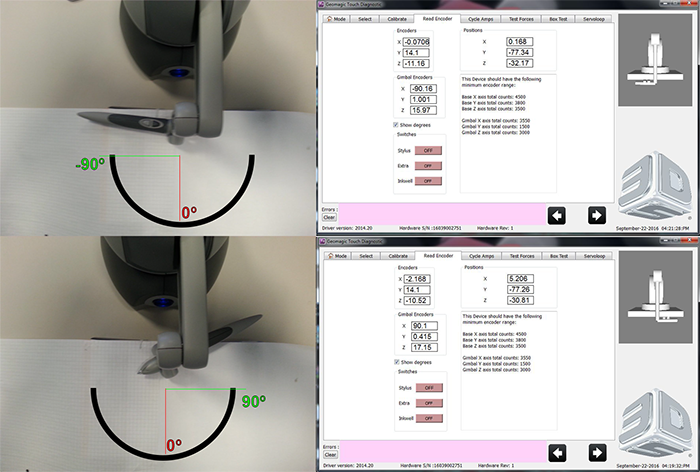
\includegraphics[width=0.5\linewidth]{IMG/errorhaptic.png}
\caption{\label{fig:errorhaptic}Diferencias de rotaciones reales frente a las proporcionadas por el dispositivo a través de su herramienta de calibración.}
\end{figure}

Con la esperanza de una solución, se contactó con la empresa que ha distribuido los dispositivos. La empresa detectó este mismo error en los dispositivos de nueva facturación y comunicó que propondrían una solución para ello. Esta solución no ha llegado en un tiempo razonable en la que permitiera proceder a la evaluación del prototipo en un entorno clínico. A su vez, se propusieron alternativas para los dispositivos, como por ejemplo utilizar solo \ac{tracker}s sacrificando la retroalimentación háptica, la cual era un punto fundamental del proyecto. Debido a la conclusión del proyecto y por tanto la falta de recursos económicos no se ha podido completar ninguna alternativa en el tiempo necesario para realizar una validación en un entorno clínico.




